\section{Design}

FlashMatrix is a general-purpose data analysis framework that provides
matrix-oriented programming interface. The architecture of FlashMatrix
is shown in Figure \ref{fig:arch}. It provides a very small set of
generalized vector and matrix operators and implements a large number of
vector and matrix operators in R with the generalized operators. The generalized
operators can be executed on each of the data containers supported by
FlashMatrix. The optimizer in FlashMatrix merges multiple operators to
reduce I/O access and achieve better parallelization.

FlashMatrix stores large data containers on SSDs through SAFS \cite{safs},
a user-space filesystem for a large SSD array, to fully utilize high I/O
throughput of the SSDs. For most of the operations, FlashMatrix accesses
data in a data container sequentially to maximize I/O throughput of SSDs.
FlashMatrix keeps some of the large data containers in memory to effectively
utilize memory in a large-RAM machine.

\begin{figure}
\centering
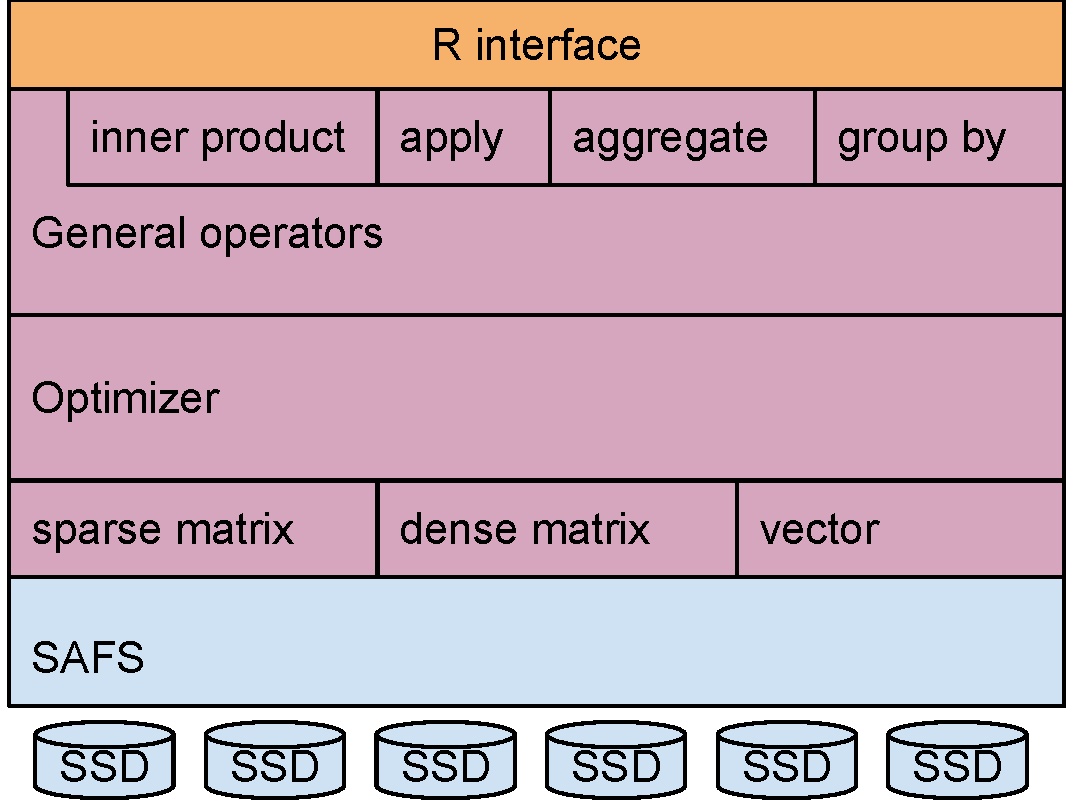
\includegraphics[scale=0.3]{./architecture.pdf}
\vspace{-5pt}
\caption{The architecture of FlashMatrix.}
\vspace{-5pt}
\label{fig:arch}
\end{figure}

\subsection{Data containers}
FlashMatrix supports two basic types of R data containers: \textit{vector}
and \textit{matrix}.
By default, FlashMatrix stores vectors in memory and matrices on SSDs with
an assumption that a matrix requires much larger storage space.
%In addition, it also
%supports two types of more advanced data containers: \textit{vector of vectors}
%and \textit{data frame}, constructed from \textit{vector}.
% We need to support sparse vector, set and map.
FlashMatrix supports both dense matrices and sparse matrices.
%	\item A \textit{vector of vectors} is a more restricted variant of R
%	\textit{list} and requires each vector has the same element type. A row-major
%	matrix can be viewed as a special \textit{vector of vectors} with each
%	vector of the same length.
%	\item A \textit{data frame} is a collection of vectors and each vector can
%	have arbitrary element types. All vectors in a data frame has the same length.
%	A column-major matrix can be viewed as a data frame with each vector of
%	the same element type.

Each type of data containers has two variants: local containers and global
containers. A global container stores data on SSDs and supports varieties of
generalized computation operators in Section \ref{sec:generalized}. A local
container is created by a generalized computation operator in a thread and
is exposed to a vectorized user-defined function (VUDF). In a machine with
non-uniform memory architecture (NUMA), the data in a local container is stored
in local memory to increase data locality.

To achieve better performance, FlashMatrix optimizes matrices of different
shapes differently. The current implementation of FlashMatrix specifically
optimizes matrix operations on two types of matrices: square sparse matrices
and tall-and-skinny (TAS) dense matrices.

%\begin{figure}
%	\centering
%	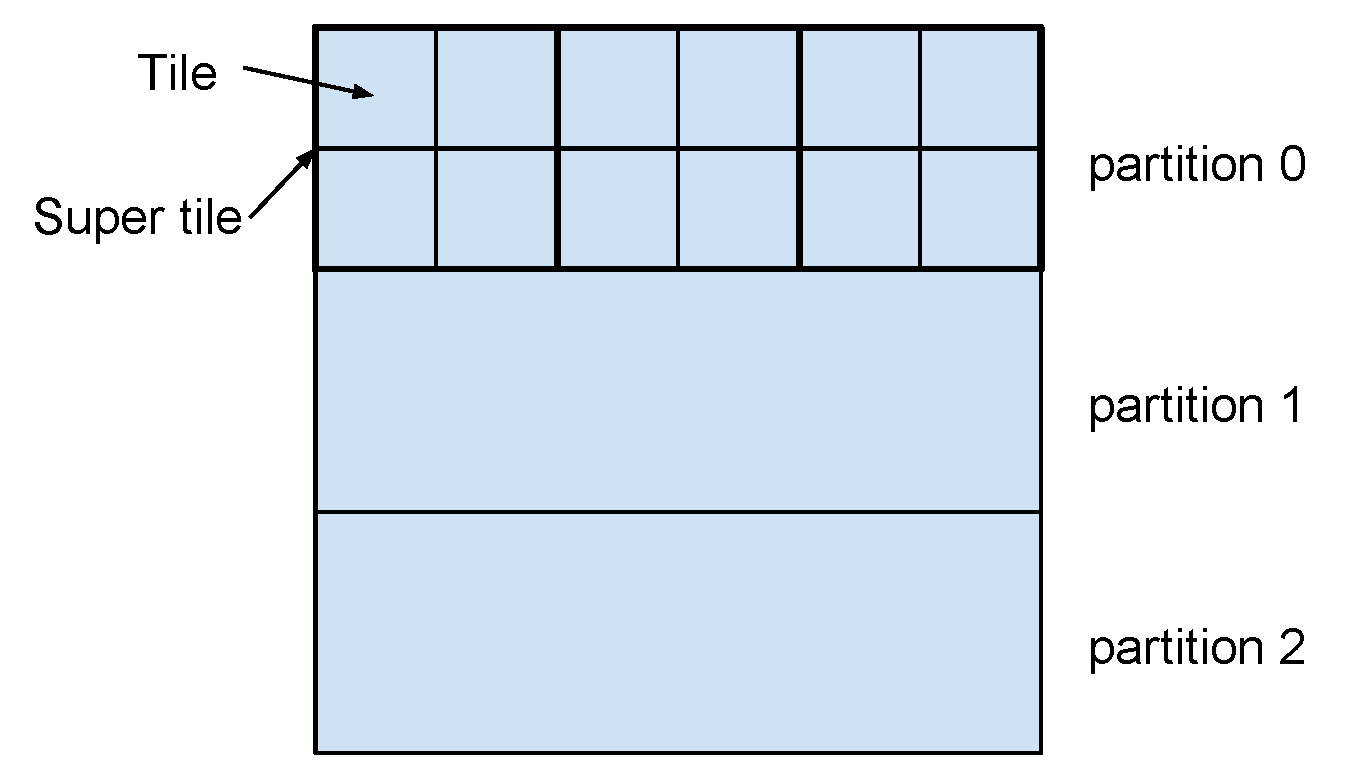
\includegraphics[scale=0.3]{./sparse_mat.pdf}
%	\vspace{-5pt}
%	\caption{The format of a sparse matrix.}
%	\vspace{-5pt}
%	\label{fig:sparse_mat}
%\end{figure}

\begin{figure}
	\centering
	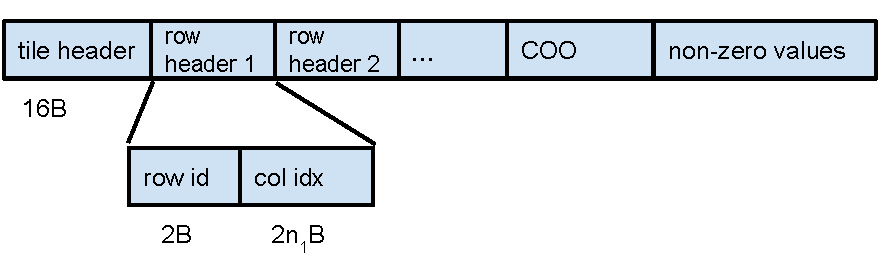
\includegraphics[scale=0.5]{./tile_format.pdf}
	\vspace{-5pt}
	\caption{The format of a tile in a sparse matrix.}
	\vspace{-5pt}
	\label{fig:tile}
\end{figure}

Sparse matrices are commonly used to represent sparse graphs, whose edge 
attributes are stored as non-zero entries in a sparse matrix. A commonly
used operation on a sparse matrix for graph analysis is sparse matrix
multiplication, so we design the sparse matrix format to specifically
optimize efficient sparse matrix multiplication. We split a sparse matrix
into small tiles for cache blocking. The size of a tile is $32K \times 32K$
at maximum and is usually
smaller, so that we can use two bytes to represent a row index or a column
index. Inside a tile, we combine SCSR (Super Compressed Row Storage) and
COO (coordinate format) to store non-zero entries to achieve more compact
data format and more efficient sparse matrix multiplication (Figure
\ref{fig:tile}). For a binary sparse matrix, non-zero values in a tile
do not need to be stored. For an asymmetric sparse matrix, we store both
the sparse matrix and the transpose of the matrix physically on SSDs.

\begin{figure}
	\centering
	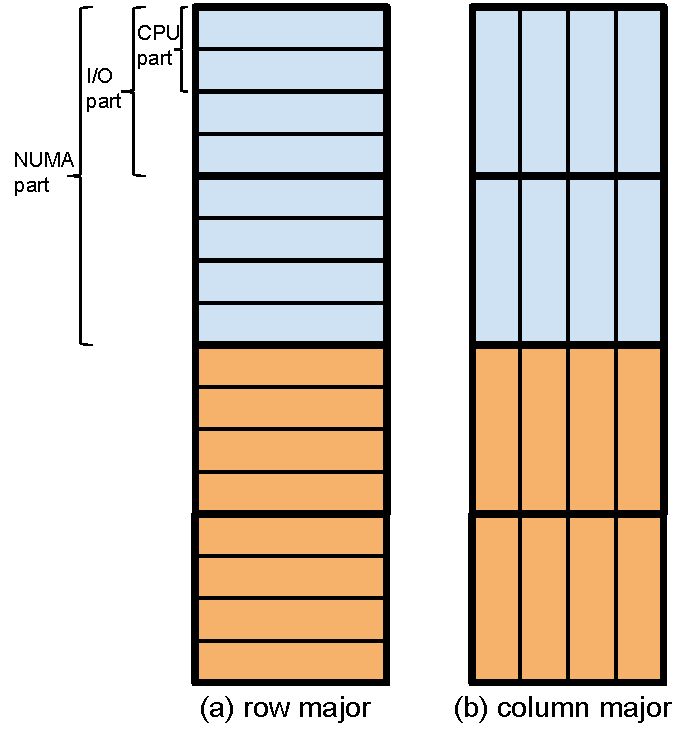
\includegraphics[scale=0.5]{./dense_matrix.pdf}
	\vspace{-5pt}
	\caption{The format of a dense matrix.}
	\vspace{-5pt}
	\label{fig:tas_mat}
\end{figure}

Tall-and-skinny (TAS) dense matrices commonly exist in many data mining
algorithms at a large scale. As suggested by their name, these matrices have
one of the dimensions much larger than the other dimension (Figure
\ref{fig:tas_mat}). For example, we use these dense matrices to store a large
set of data points with a small number of features. FlashMatrix supports both
row-major and column-major matrices to avoid physical data copy for some matrix
operations such as matrix transpose. The layout of a matrix is generally
determined by a FlashMatrix operation but can also be determined by users. 
For parallelization and efficient data access, these dense matrices are
partitioned horizontally and all elements in a partition are stored in a piece
of contiguous memory. As such, a column in a column-major TAS matrix is not
stored contiguously.

%\subsection{Basic operations} \label{sec:basic}
%create a data container

%data container conversion

%matrix operations: convert data layout and transpose.

%append an element to a vector can be implemented as physically appending the element
%to the vector. The result vector becomes the new vector, and the original vector
%becomes the sub-vector of the new vector.

\subsection{Generalized computation operations} \label{sec:generalized}
To enhance the flexibility and simplify the implementation, FlashMatrix only
provides a small set of generalized operators on vectors and matrices.
The current implementation has four generalized operators: \textit{inner product},
\textit{apply}, \textit{aggregation} and \textit{groupby}. Each operator
accepts user-defined functions (UDF). Like most of R functions, these operators
do not change data in the input data containers and each operation generates
a new data container.

\textit{Inner product} is a generalized matrix multiplication. It replaces
multiplication and addition in matrix multiplication with two user-defined
functions, respectively. As such, we can define many operations with inner
product. For example, we can use inner product to compute various pair-wise
distance matrics of vectors such as Euclidean distance \cite{euclidean} and
Hamming distance \cite{hamming}. We can also apply inner product to sparse
matrices to compute PageRank, belief propagation, etc.
Even though we can implement matrix multiplication with inner product,
FlashMatrix still relies on BLAS to implement matrix multiplicatoin for
float-point matrices to achieve speed and float-point precision required by
many numeric libraries such as the Trilinos eigensolver \cite{anasazi}.

\textit{Apply} is a generalized form of element-wise operations and has
multiple variants. The simplest form of \textit{apply}, denoted with
\textit{sapply}, is a generalized element-wise unary operation whose
UDF takes an element in a vector or a matrix at a time and outputs a value.
We can use it to implement unary operations such as negation, square root
or type casting of individual elements in a vector or a matrix. The second
form of \textit{apply}, denoted with \textit{mapply2}, is a generalized
element-wise binary operation whose UDF takes an element from each vector
or matrix and outputs a single value. We use it to implement many binary
matrix operations such as matrix addition and subtraction. The third form of
\textit{apply}, denoted by \textit{apply\_mat}, is a generalized row-wise or
column-wise operation whose UDF takes a row or a column at time and outputs
a vector of elements.

\textit{Aggregation} takes multiple elements and outputs a single element.
It has two forms on matrices. The first form, denoted by \textit{agg\_arr}
aggregates over all elements on a matrix. Operations such as summation and
maximum are special cases of the first form. The second form, denoted by
\textit{agg\_mat} aggregates over each individual row or column.
Row sum and column sum are special cases of the second form.

\textit{Groupby} takes a vector of elements along with a vector of categorical
values and invokes UDF on the elements associated with the same categorical
value. \textit{Groupby} also works on a matrix if we view a matrix as a vector
of vectors.

The function of some of the operators overlaps. For example, \textit{apply\_mat}
is a generalized form of \textit{agg\_mat}, but \textit{agg\_mat} can be
implemented more efficiently. Therefore, FlashMatrix provides both operators.

%TODO applying the operators to a sparse matrix.

\subsection{Vectorized user-defined function}
UDF potentially introduces significant computation overhead. Traditionally,
UDF is applied to every individual element in a data container and, thus,
the computation on every element suffers from the large overhead of a function
call. Therefore, relying on UDF to implement commonly used vector and matrix
operations reduces the performance of the entire system significantly.
We need to highly optimize UDF to achieve the same performance as
the specialized matrix operations.

To amortize the overhead of function calls, all generalized operators take
vectorized user-defined functions (VUDF), which operates on an array of elements
instead of individual elements. The number of elements in an invocation of
VUDF determines how much overhead is amortized. However, too many elements
in one invocation potentially increase CPU cache misses when the computation
is constructed in a DAG shown in Section {}. For the elements of primitive
types, the number of elements in one invocation of VUDF can be as large as 1000,
which can still perfectly fit in the L1 CPU cache.

The generalized operators require multiple forms of VUDF. The first form takes
two arrays with the same number of elements and outputs an array of the same
length as the input arrays. The second form takes one array of elements and
a single element and outputs an array of the same length as the input array.
The first two forms are essential for binary operations such as
\textit{inner product} and \textit{mapply2} as well as \textit{agg\_mat} and
\textit{groupby\_mat}.
The third form takes an array of elements and outputs an array of the same
length, which is essential for \textit{sapply}.
The fourth form takes an array of elements and outputs a single element,
which is essential for \textit{aggregation}.

FlashMatrix has many commonly used VUDFs implemented in the framework by default.
These VUDFs wrap basic operations built in many programming languages and
libraries. For example, FlashMatrix provides arithmetic operations such as addition
and subtraction, relational operations such as equal to and less than, logical
operations such as logical AND and logical OR, as well as commonly used
math functions such as computing absolute values and square root. FlashMatrix
also provides a set of VUDFs to cast primitive element types. The built-in
binary operation usually needs to support three forms: form1, form2 and form3,
while the unary operation only needs to support form3. In addition, built-in
VUDFs also need to support different element types. Thus, each basic operation
supported by FlashMatrix has multiple VUDF implementations.

%TODO We can compose a VUDF with basic VUDFs to perform more complex tasks.
%memory buffer allocation for VUDF

To reduce the number of VUDF implementations for different element types, form1
and form2 require the input elements to have the same type. If a generalized
operator gets two data containers with different element types, it first casts
the type of the elements in one container to match the element type of the other
container. Type casting follows the usual arithmetic conversions \cite{}
commonly seen in many programming languages. The type casting is performed
laziy and no additional data container is generated in type casting
(in Section \ref{sec:lazy_eval}).

For easier parallelization, generalized operators assume that VUDF is stateless.
Therefore, the generalized operators carry the mutable state of the computation.
However, VUDF can carry immutable values to simplify some implementations.

\subsection{Memory management}

% TODO A more dynamic caching. We need to dynamically determine when and
% which part of data should be cached.

Having a per-thread buffer to store data read from SSDs or materialized from
a virtual matrix.

When materializing a large matrix in memory, we need to allocate large pieces
of memory for the matrix. Linux uses \textit{mmap} to allocate large memory
and populate the allocated memory with physical pages via page fault when
the memory is touched for the first time. As such, it is expensive to allocate
large memory in Linux. As such, we maintain memory buffers with physical pages
populated in advance.

Because VUDF runs on an array of elements, we need to allocate a temporary
memory buffer to store the intermediate computation results.
VUDF requires data always in CPU cache.

\subsection{Lazy evaluation} \label{sec:lazy_eval}
Lazy evaluation avoids materializing every data container to reduce I/O.
With lazy evaluation, an operator outputs a special matrix to represent
the operation result and this special matrix does not store the actual data of
the operation result. Instead, it stores the computation and a reference to
the input matrices. We refer to these special matrices as
\textit{virtual matrices}.

The current implementation of FlashMatrix applies lazy evaluation to multiple
generalized operators on certain data containers. Lazy evaluation can be easily
applied to \textit{sapply} and \textit{mapply}. It is applied to \textit{apply\_mat}
and \textit{agg\_mat} when these two operators runs on rows of a TAS matrix.
It is also applied to \textit{inner product} when \textit{inner product} runs
on a TAS matrix and a small matrix. In general, lazy evaluation is currently
only applied to operators that output large data containers to reduce the amount
of data written to SSDs.

By default, FlashMatrix materializes a \textit{virtual matrix} as late as
possible to increase saved I/O, especially writes. However, this strategy
may have the cost of increasing computation or even increase the number of
reads. As such, we allow users to explicitly force FlashMatrix to materialize
a \textit{virtual matrix} when necessary.

% TODO users can choose whether FlashMatrix should keep the materialized result.
% For apply, we can usually materialize its result on the fly since this operation
% is usually cheap. But we might want to keep the result of inner product.

% TODO lazy evaluation on sparse matrix multiplication.

%With \textit{virtual matrices}, we construct a directed acyclic graph (DAG)
%at runtime to represent computation constructed in FlashMatrix. In the DAG, we
%store all scalar variables and small matrices as part of computation. Inside
%this DAG, we do not need to perform any computation other than the last one.

To enable lazy evaluation, all matrices in FlashMatrix are immutable.
As such, \textit{virtual matrices} can generate the same result every time
they are materialized. A dense matrix is garbage collected only when
there are not any references to the matrix.

A \textit{virtual matrix} may contain a sequence of operations, so materializing
it may trigger matrix materialization recursively. We discard the materialized
partition of an intermediate matrix, once it is no longer needed, to avoid
writing data of an intermediate matrix to SSDs. For a \textit{virtual matrix}
that represents a TAS matrix, we partition it horizontally in the same fashion
as a actual TAS matrix and materialize each partation independantly. To increase
CPU cache hits, we use a much smaller partition size than
the external-memory matrix. As such, the output of the previous operation is
still in the CPU cache when it is fed to the next operation.

% TODO unnamed data containers should be always virtualized data containers.

\subsection{Integration with R}

FlashMatrix provides an R extension called FlashR to seamlessly integrate with
R and power R for large-scale data mining. FlashR provides wrapper functions
for each of the generalized operators
in FlashMatrix. In addition, we implement many commonly used R functions with
the generalized operators to provide R users a familiar programming environment
while the underlying optimizer in FlashMatrix merges operations and
automatically parallelizes complex algorithms written in R.

The current implementation provides a large set of built-in VUDFs in FlashR.
Users are able to implement many R functions with these built-in VUDFs.
Users can also implement their own VUDFs in C/C++ and load to R to further
extend the capability of FlashR.

Garbage collection of vectors and matrices.

\subsection{Applications}

We implement a few well-known data mining algorithms to demonstrate
the flexibility and the performance of FlashMatrix. All of the algorithms
can be expressed with a set of vector and matrix operations. We implement
all of them with its R interface.

\begin{figure}[t]
%\begin{lstlisting}
\begin{minted}[mathescape,
		fontsize=\scriptsize,
		frame=single,
]{r}
d <- 0.85
N <- dim(A)[1]
one <- rep.int(1, N)
deg <- A %*% one
pr1 <- rep.int(1/N, N)
converge <- 0
A <- t(A)
while (converge < N) {
	pr2 <- (1-d)/N+d*A%*%(pr1/deg)
	diff <- abs(pr1-pr2)
	converge <- sum(diff<eps)
	pr1 <- pr2
}
\end{minted}
%\end{lstlisting}
\vspace{-5pt}
\caption{The implementation of PageRank.}
\label{fig:pagerank}
\end{figure}

PageRank is one of top 10 data mining algorithms identified by the IEEE
International Conference on Data Mining (ICDM) \cite{top10}. It is also
commonly used for benchmarking a graph processing framework.

\begin{figure}[t]
%\begin{lstlisting}
\begin{minted}[mathescape,
		fontsize=\scriptsize,
		frame=single,
]{r}
# trace of W %*% H
trace.MM <- function(W, H) {
	X <- W * t(H)
	sum(X)
}

# ||A - W %*% H||^2
Fnorm <- function(A, W, H) {
	tr2 <- trace.MM(t(A) %*% W, H)
	tr3 <- trace.MM(t(H) %*% (t(W) %*% W), H)
	sum(A * A) - 2 * tr2 + tr3
}

n <- dim(A)[1]
m <- dim(A)[2]
W <- matrix(runif(n*k), n, k)
H <- matrix(runif(k*m), k, m)

for (i in 1:niters) {
	# Update H
	den <- (t(W)%*%W)%*%H
	H <- pmax(H*(t(W)%*%V), eps)/(den+eps)

	# Update W
	den <- W%*%(H%*%t(H))
	W <- pmax(W*(V%*%t(H)), eps)/(den+eps)

	if (i %% 5 == 0 && Fnorm(A, W, H) < thres)
		break
}
\end{minted}
%\end{lstlisting}
\vspace{-5pt}
\caption{The implementation of NMF.}
\label{fig:pma}
\end{figure}

\begin{figure}[t]
%\begin{lstlisting}
\begin{minted}[mathescape,
		fontsize=\scriptsize,
		frame=single,
]{r}
# calculate the new centers by averaging data pointers
# in a cluster.
cal.centers <- function(data, parts) {
	n <- dim(data)[1]
	one <- rep.int(1, n)
	sizes <- groupby(one, parts, sum)
	centers <- groupby(data, parts, sum)
	centers <- diag(1/sizes) %*% centers
}

#initialize centers
n <- dim(data)[1]
m <- dim(data)[2]
rand.parts <- floor(runif(n, min=1, max=K+1))
new.centers <- cal.centers(data, rand.parts)
centers <- matrix(rep.int(0, K * m), K, m)

while (sum(centers == new.centers) == length(centers)) {
	centers <- new.centers
	m <- inner.prod(data, t(centers), dist, add)
	# calculate the new center of each data pointer.
	dp.centers <- apply(m, 1, which.min)
	new.centers <- cal.centers(data, dp.centers)
}
\end{minted}
%\end{lstlisting}
\vspace{-5pt}
\caption{The implementation of KMeans.}
\label{fig:kmeans}
\end{figure}

% TODO each KMeans iteration only needs to read the entire data matrix once.
